\entry{Semana del 08/12/2025} 
Esta semana (y parte de la anterior) la dediqué a analizar las series temporales resultantes de la última medición. 



\section{Espectros temporales de las señales} 
Lo primero que hice con las señales fue usar el algoritmo de Welch con los mismos parámetros que venía usando para encontrar las PSDs y ver los espectros. 


\begin{figure}[!ht]
	\begin{minipage}[c]{0.5\textwidth}
			\begin{subfigure}{\textwidth}
					\centering
					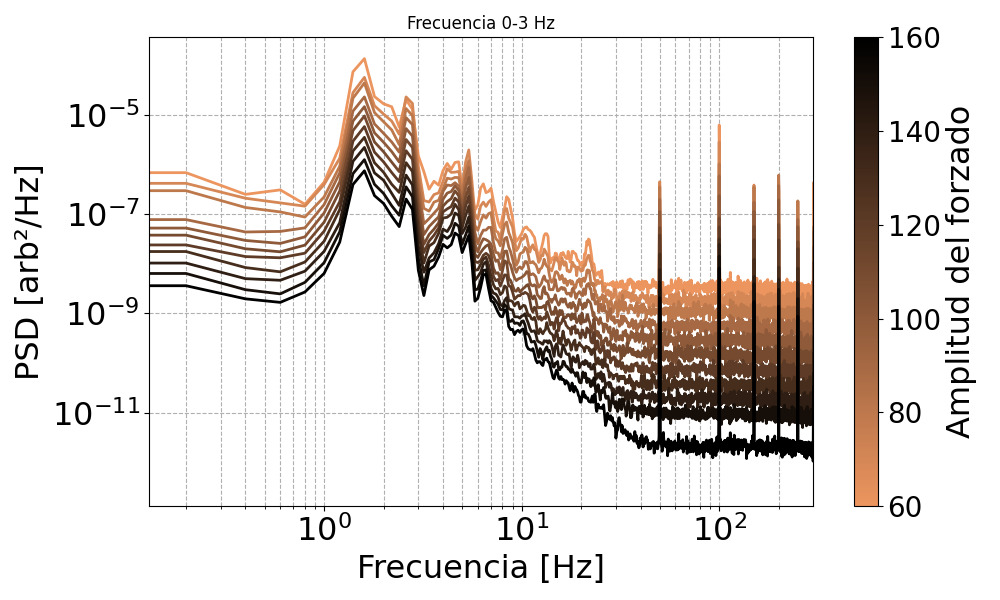
\includegraphics[width=0.98\textwidth]{Figures/01_12_2025/Espectros_0_3}
					\captionsetup{width=0.8\textwidth}
					\subcaption{0-3 Hz.}
				\end{subfigure}
		\end{minipage}\begin{minipage}[c]{0.49\textwidth}
			\begin{subfigure}{\textwidth}
					\centering
					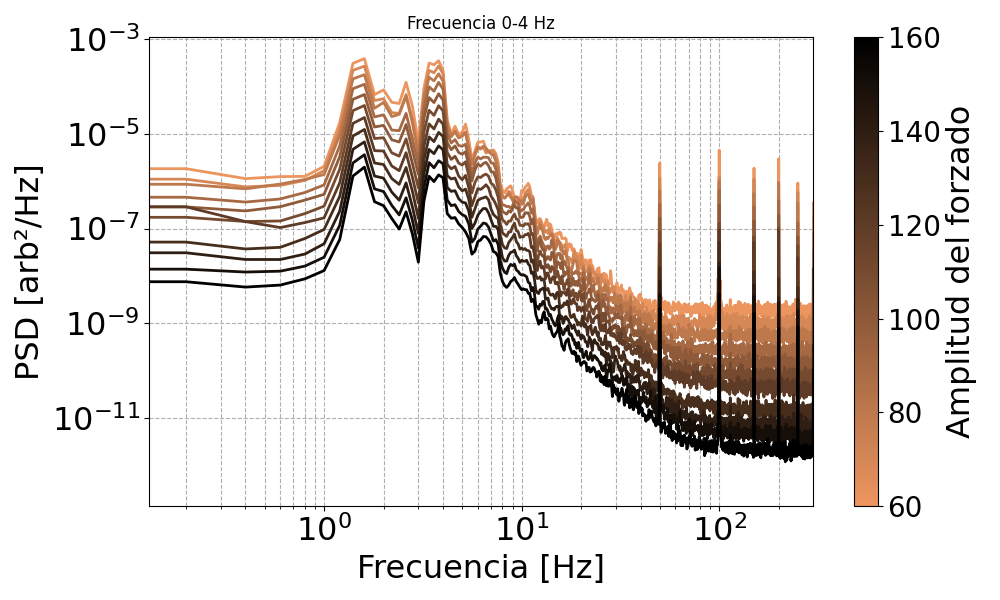
\includegraphics[width=0.98\textwidth]{Figures/01_12_2025/Espectros_0_4}
					\captionsetup{width=0.8\textwidth}
					\subcaption{0-4 Hz.}
				\end{subfigure}
		\end{minipage} 
		
		\begin{minipage}[c]{0.5\textwidth}	
			\begin{subfigure}{\textwidth}
				\centering
				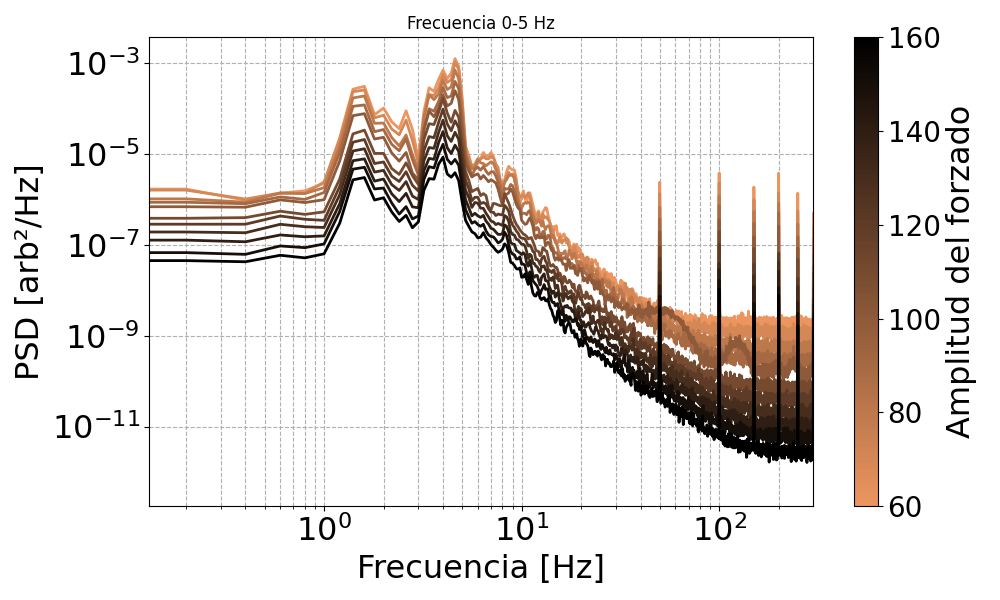
\includegraphics[width=0.98\textwidth]{Figures/01_12_2025/Espectros_0_5}
				\captionsetup{width=0.8\textwidth}
				\subcaption{0-5 Hz.}
			\end{subfigure}
		\end{minipage}\begin{minipage}[c]{0.49\textwidth}
			\begin{subfigure}{\textwidth}
				\centering
				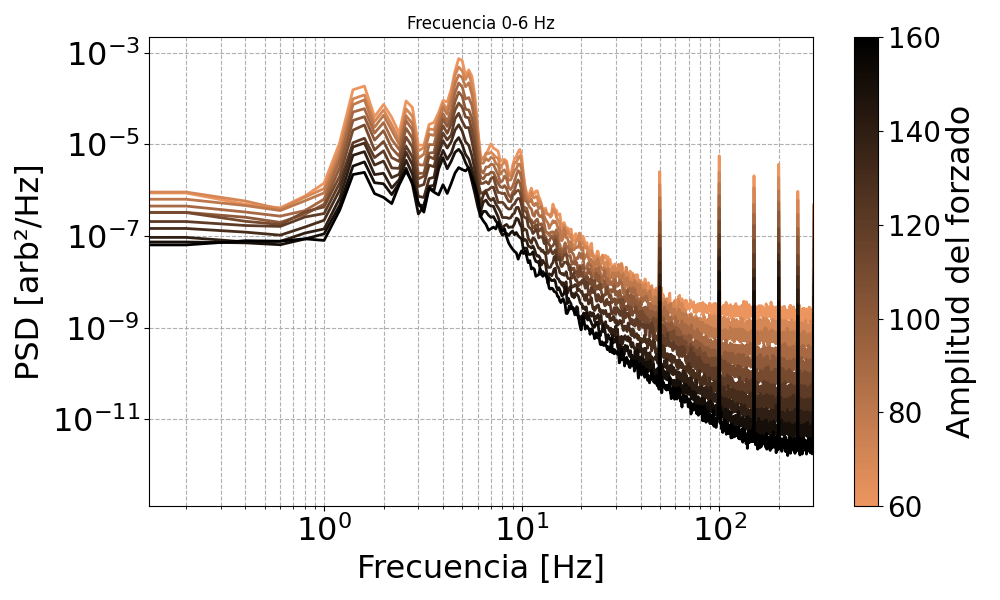
\includegraphics[width=0.98\textwidth]{Figures/01_12_2025/Espectros_0_6}
				\captionsetup{width=0.8\textwidth}
				\subcaption{0-6 Hz.}
			\end{subfigure}
		\end{minipage} 
	\caption{PSDs para las mediciones en las distintas bandas de frecuencias.}
	\label{fig:espectros_sistemáticos} % fig:03 
\end{figure}

De estos espectros se nota que se va agrandando la cascada hasta el cutoff a medida que aumenta la energía inyectada. Además podemos ver que los picos de frecuencias bajas se corresponden en cada caso con el rango de frecuencias usados para el forzado, empezando la cascada después de eso. 

Las ondas que no estamos 100 \% seguros de qué son aparecieron en una sola de las mediciones para la banda de 0-5 Hz (curiosamente la vez pasada también habían aparecido en esta banda). 


\section{Parámetros de las cascadas } 
Después de haber calculados los distintos espectros la idea sería encontrar los distintos parámetros que los caracterizan. Éstos serían las pendientes del rango capilar y de gravedad, la frecuencia de cruce entre ambos (codos) y el cutoff. 

Para hallar el cutoff lo que estoy haciendo es calcular en frecuencias altas el valor medio (por ejemplo entre 200-250 Hz) y su desviación estándar. Luego me fijo el quinto punto del espectro que cruza la línea a 0.3 veces el desvío estándar. Tomé 0.3 veces en vez de 1, y el quinto punto en vez del primero, ya que esta combinmación me asegura no cortar por el ruido parte de la cascada. Estos valores salieron de hacer pruebas de a poco e ir revisando el cutoff resultante para los distintos espectros, hasta hallar esos que funcionan bien para todos.  

\begin{figure}[th!]
	\centering
	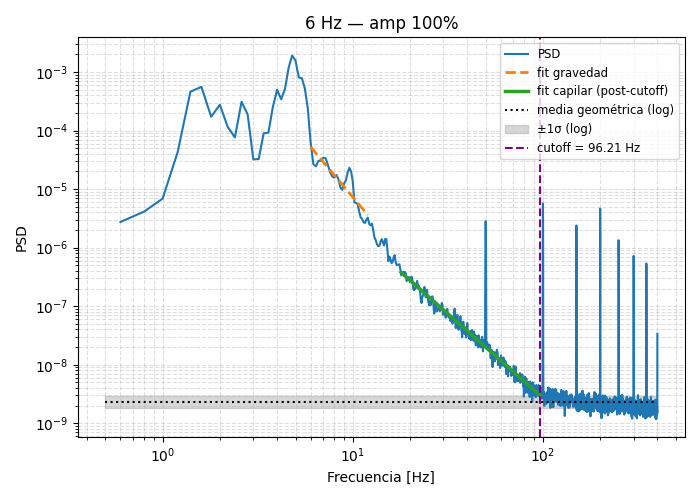
\includegraphics[width=0.54312689017\linewidth]{Figures/01_12_2025/Ejemplo_rango_dinámico_para_los_ajustes}
	\caption{Esquema de cómo se detectó el cutoff en las PSDs. }
	\label{fig:ejemplorangodinamicoparalosajustes}
\end{figure}

Para hallar los exponentes probé dos cosas. En un primer lugar elegir los rangos para ajustar el espectro linealmente a mano como lo hice originalmente, con la única diferencia de que el rango de gravedad lo ajusto hasta el cutoff. % esto 

Los resultados son los siguientes: 
\begin{figure}[th!]
	\centering
	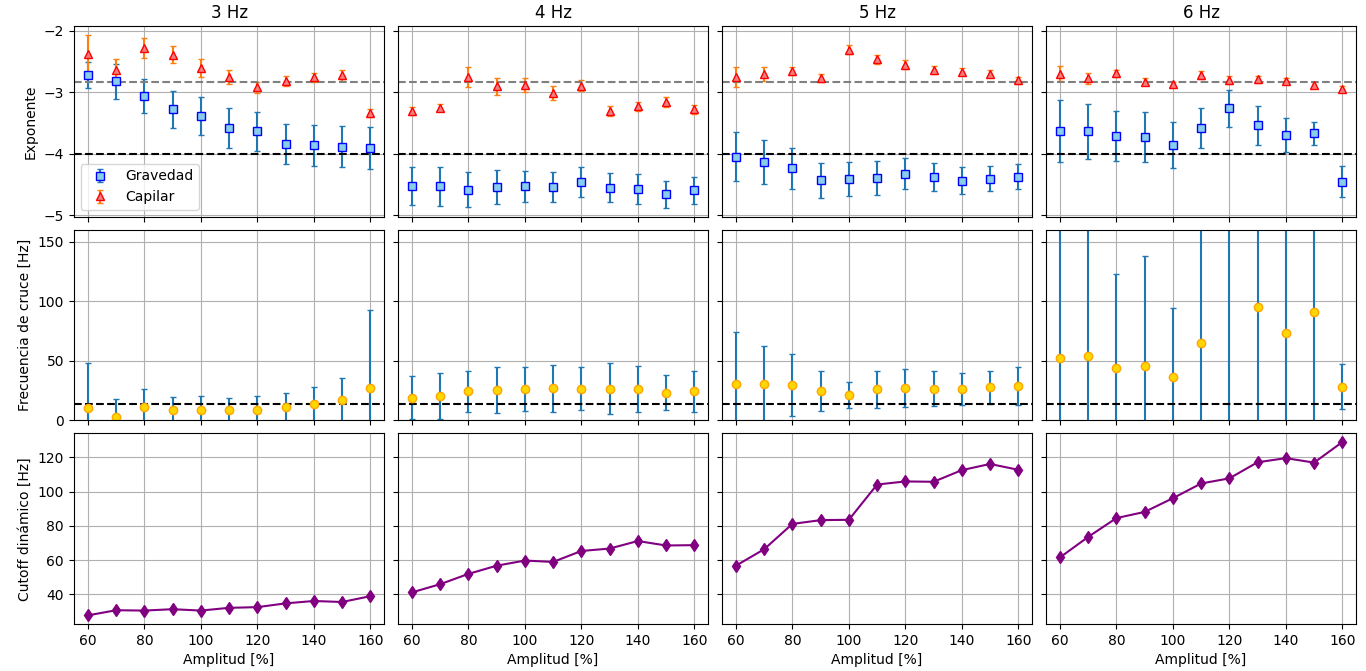
\includegraphics[width=0.97\linewidth]{Figures/01_12_2025/Gráfico_TOTAL_v2_completo_FINAL}
	\caption{Parámetros de las cascadas eligiendo el rango de ajuste \textit{a mano}.}
	\label{fig:graficototalv2completofinal}
\end{figure}

Podemos ver que el cutoff crece a medida que aumenta la energía inyectada, llegando cada vez más lejos la cascada. Además los exponentes de capilaridad dan muy cercanos al teórico (más que antes). El de gravedad alcanza -4 hacia el final de la primera banda (0-3 Hz) y después se mantiene al rededor de -4.5 (cerca del -5 que sería el de Phillip en los océanos). Lo único que da con muchísimo error es la frecuencia de corte. 

Para tratar de evitar posibles críticas al método de elegir el rango de ajuste (y tratar de mejorar la determinación de las frecuencias de cruce) lo que hice fue ajustar con una función partida de dos lineales. Tenemos cuatro parámetros libres, $a_1$ y $b_1$ de la primera lineal, $a_2$ de la segunda y $f_c$ de la unión ($b_2$ sale de pedir continuidad). Por lo que estuve viendo hay paquetes de Python ya escritos para este tipo de ajustes (linear regression with breakpoints) que podría probar. Además el rango del ajuste es desde el final de la banda del forzado hasta el cutoff, con lo cual abarca la cascada en su totalidad.  

Los resultados fueron los siguientes: 

\begin{figure}[th!]
	\centering
	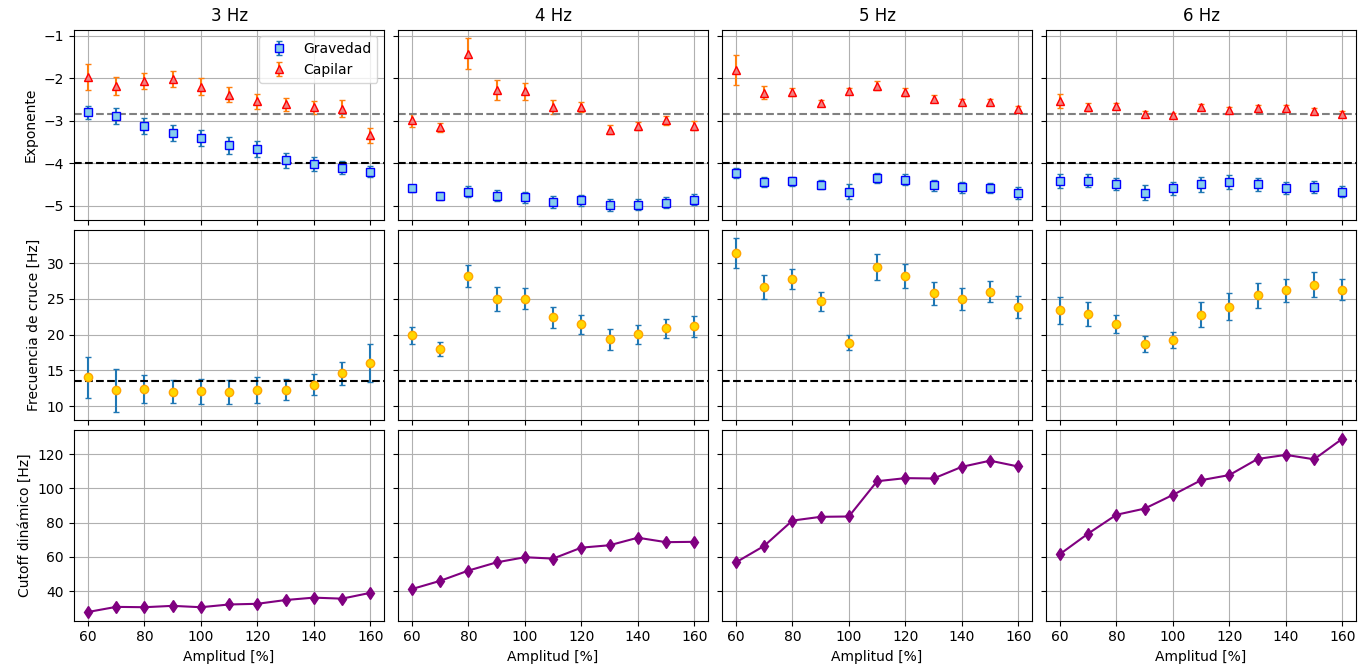
\includegraphics[width=0.97\linewidth]{Figures/01_12_2025/Gráfico_TOTAL_función_partida_v2}
	\caption{}
	\label{fig:graficototalfuncionpartidav2}
\end{figure}

Para los exponentes dio bastante parecido, solo que con menos error, y ahora sí dio bastante mejor la frecuencia de cruce. En 0-3 Hz se mantiene siempre compatible con 13.5 Hz y después va aumentando como le pasa a \cite{falconObservationGravityCapillaryWave2007}. En ambos casos parece que tendiera al doble de frecuencia (acá sería 27 Hz y para ellos 34 Hz en el mercurio).  

Para la banda de 0-3 Hz (si solo mirásemos esa pensando que es la única verdaderamente débilmente no lineal) tienden los exponentes bien a sus valores teóricos. 

Los primeros puntos de la banda de 0-4 Hz y algunos pocos otros hacen cosas raras porque dejan un rango muy chico de capilar y no llega a ajustar bien (habría que restringir los parámetros para que no se acerce tanto $f_c$ a la frecuencia del cutoff).  

\section{Wave Steepness} 
\subsection*{Ondas regulares. } 

El parámetro que nos habla de la no linealidad del sistema es el \textit{wave steepness} ($S$), que para una onda regular se define como: 

\begin{equation}
	S = \frac{H}{L} 
\end{equation}

Donde $H$ es la altura desde el valle de la onda hasta su cresta, y $L$ la longitud de onda. Si tenemos señales temporales podemos hallar $L(T)$ utilizando la relación de dispersión que corresponda, siendo $T$ el período de las olas. 

\subsection*{Ondas irregulares. } 

En nuestro caso no tenemos ondas regulares, sino una mezcla de ondas en muchas direcciones. Siguiendo lo que hacen en \cite{tayfunDistributionsWaveSteepness2006} podemos definir un steepness medio. Para esto lo que vamos a hacer es separar la señal en ondas individuales mediante la detección de \textit{zero-crossings}. 

El procedimiento consiste en detectar los puntos donde la señal calibrada (ya que nos interesa ahora sí el valor de la altura) cruza cero (cambia de signo). Para la calibración usé los parámetros que salieron de la última calibración con el motor (Miércoles 10/09/2025\footnote{NOTA IMPORTANTE: en la función trim del lockin estaba mal el factor multiplicativo, debería ser al cuadrado.}), y le resté el valor medio que depende de la frecuencia elegida (solo quedaría en cero si pudiésemos poner perfectamente la de resonancia, sino queda un $\phi_0$ arbitrario, además del desfasaje exacto entre los canales del sensor, o sea, los puntos donde sampleamos la referencia y la señal). 

\begin{figure}[th!]
	\centering
	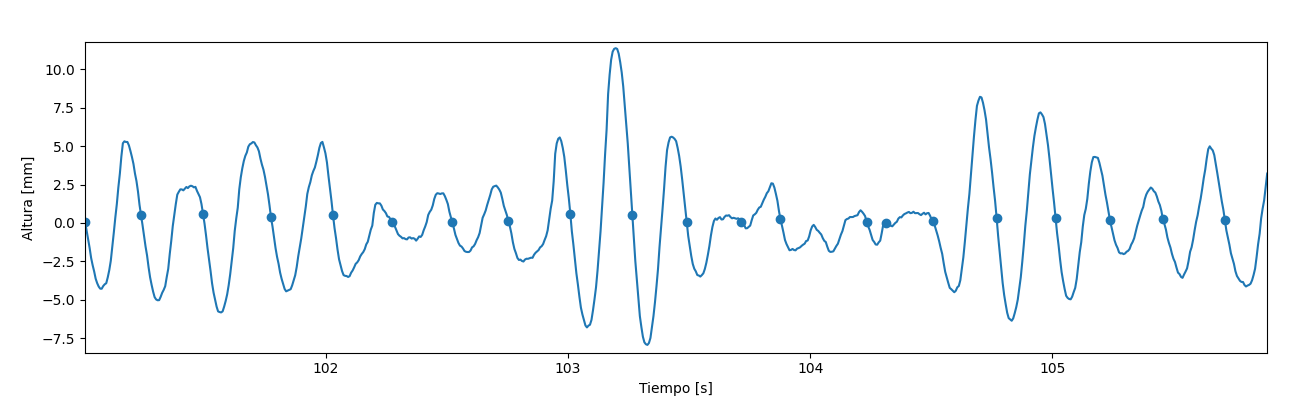
\includegraphics[width=0.87\linewidth]{Figures/08_12_2025/Individual_wAves}
	\caption{Esquema de las ondas individuales.}
	\label{fig:individualwaves}
\end{figure}

Como hacen en \cite{francisSynopticForcingWave2012}, los parámetros de cada onda individual se definen como $H_i=\max\{h_i \} - \min\{h_i\}$, con $h_i$ la serie temporal para esa onda individual (entre dos cruces de cero en el mismo sentido), y $T_i$ es la duración de $h_i$. % diferencia de tiempo entre donde

De esta forma tendremos un conjunto de puntos $(T_i, H_i)$. Con éste podemos ver dos cosas, la distribución conjunta de altura y período, y la distribución de probabilidad de $S$. Para cada señal tenemos unas 150-200 ondas individuales aproximadamente. 
 
 
\subsection*{Distribución conjunta} 
Lo primero a ver es la nube de puntos que obtenemos para cada una de las ondas individuales. Un gráfico de ejemplo donde se muestran también las curvas de nivel para la densidad de puntos (con KDE Gaussian) es el siguiente: 

\begin{figure}[th!]
	\centering
	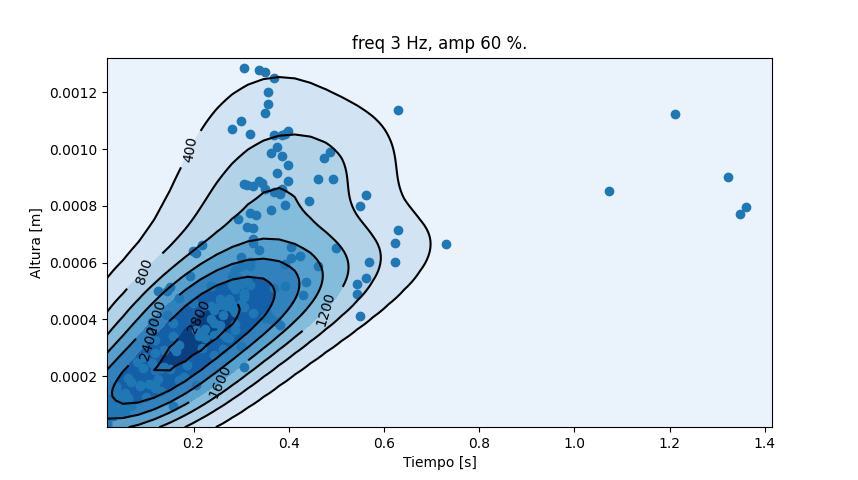
\includegraphics[width=0.7\linewidth]{Figures/08_12_2025/joint_level_curves}
	\caption{Gráfico para la densidad 2D del conjunto de puntos $(T_i, H_i)$ de las ondas individuales. } 
	\label{fig:jointlevelcurves}
\end{figure}

Si vemos lo que pasa para los demás datos tenemos la siguiente progresión. 
\begin{figure}[!ht]
	\centering
	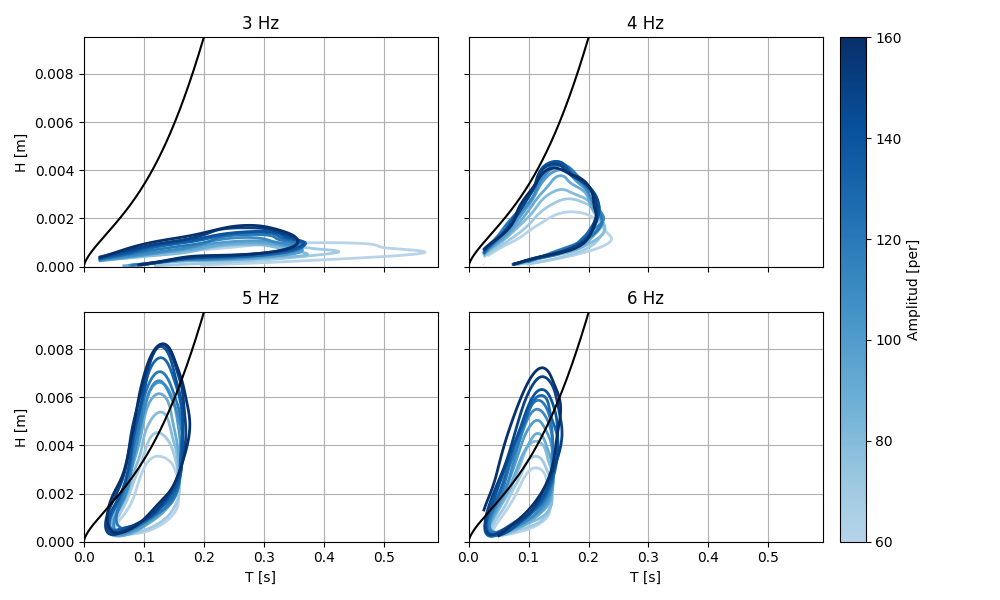
\includegraphics[width=0.7\linewidth]{Figures/08_12_2025/Progresión}
	\caption{}
	\label{fig:progresion}
\end{figure}

Donde las curvas graficadas se corresponden con la curva de nivel que encierra al 67 \% de los puntos. 

La línea sólida se corresponde con lo que sería el steepness máximo correspondientes a ondas de Stokes (en la teorpia lineal): 

\begin{equation}
	S_{text{lím}} = \frac{H_{\text{máx}}}{L(T)} \approx \frac{1}{7} \tanh{k(T)d} 
\end{equation}

Donde $d=(4.45\pm0.05)$ cm es la altura del agua en la cuba. Eventualmente para el caso donde ya no es tan débilmente no lineal se cruza esta línea de altura máxima y tenemos más steepness incluso (entraríamos en strong turbulence). Me gustaría realizar mediciones específicamente dedicadas a esto con el factor de calibración bien determinado por las dudas (o estimar la gravedad con el sensor sin calibrar, o bien usar los datos de este mapa para hallar el factor de calibración si suponemos que su límite es la línea).  

Una cosa interesante es que si normalizamos las nubes de puntos por sus valores medios en ambos ejes se colapsan todas y terminan siendo iguales. La cuestión es que al tener todas distintos valores medios no está bien graficarlas usando los mismos ejes, eso me queda la duda. 

\subsection*{Distribución de $S$} 
Otra cosa que podemos hacer es ver la distribución de $S_i$ de la serie de ondas individuales. A modo de normalización vamos a analizar lo que pasa con $S_i/S_{\text{rms}}$, y esto además nos saca (si los hubiese) problemas en el factor de calibración. Éste factor es simplemente: 

\begin{equation}
	S_\text{rms}^2 = \langle\frac{H_i}{L(T_i)}\rangle^2 
\end{equation}

Y algunas de las distribuciones son las siguientes: 


\begin{figure}[!ht]
	\begin{minipage}[c]{0.325\textwidth}
			\begin{subfigure}{\textwidth}
					\centering
					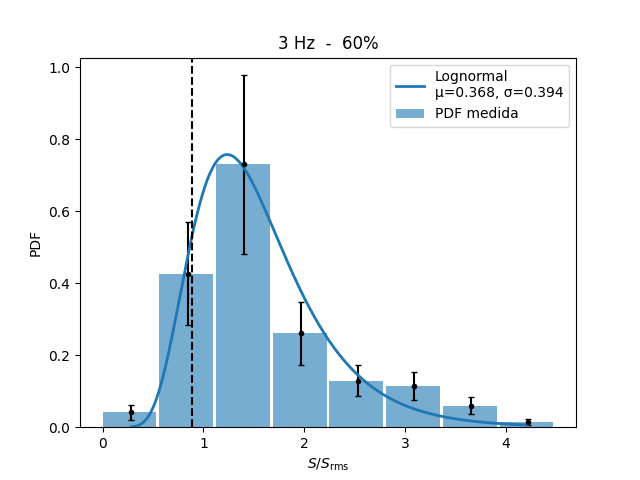
\includegraphics[width=0.98\textwidth]{Figures/08_12_2025/Distribuciones log-normal full/1}
					\captionsetup{width=0.8\textwidth}
					\subcaption{}
				\end{subfigure}
		\end{minipage}\begin{minipage}[c]{0.3249\textwidth}
			\begin{subfigure}{\textwidth}
					\centering
					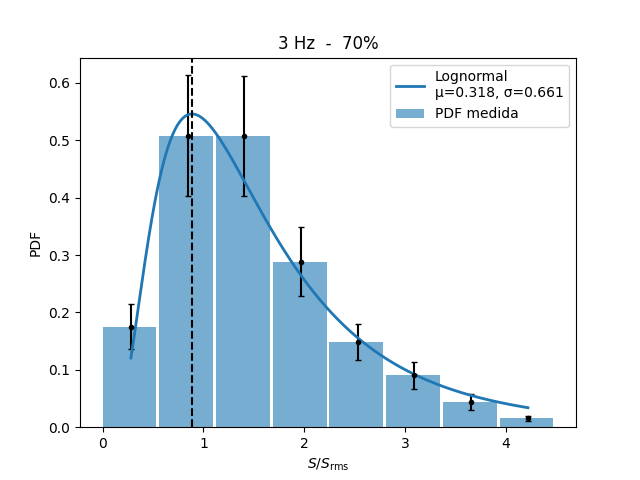
\includegraphics[width=0.98\textwidth]{Figures/08_12_2025/Distribuciones log-normal full/2}
					\captionsetup{width=0.8\textwidth}
					\subcaption{}
				\end{subfigure}
			\end{minipage}\begin{minipage}[c]{0.325\textwidth}
				\begin{subfigure}{\textwidth}
					\centering
					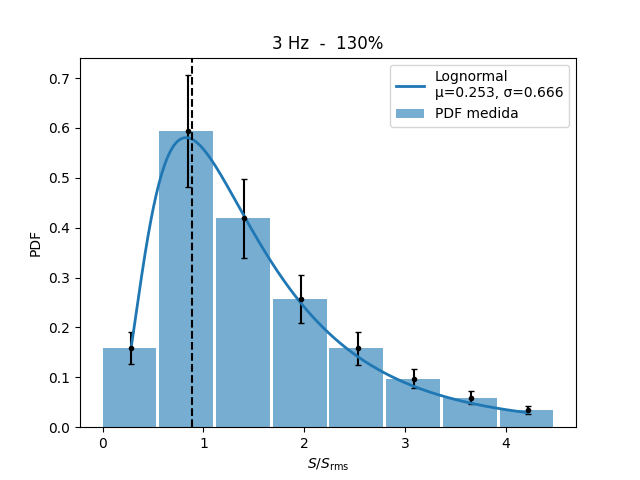
\includegraphics[width=0.98\textwidth]{Figures/08_12_2025/Distribuciones log-normal full/8}
					\captionsetup{width=0.8\textwidth}
					\subcaption{}
				\end{subfigure}
				\end{minipage}
		\begin{minipage}[c]{0.325\textwidth}
			\begin{subfigure}{\textwidth}
				\centering
				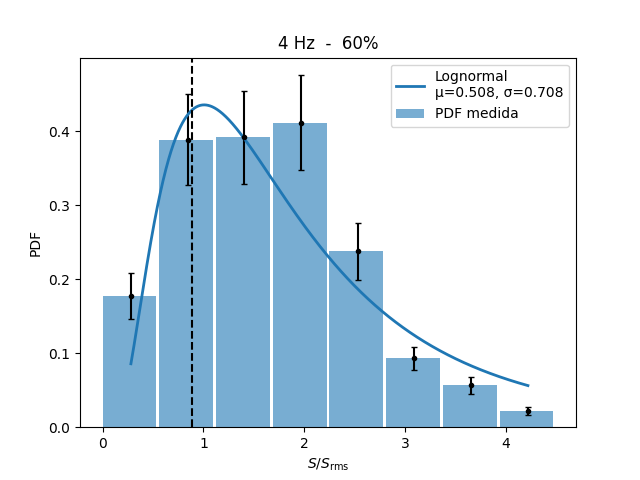
\includegraphics[width=0.98\textwidth]{Figures/08_12_2025/Distribuciones log-normal full/12}
				\captionsetup{width=0.8\textwidth}
				\subcaption{}
			\end{subfigure}
		\end{minipage}		

			
		\begin{minipage}[c]{0.325\textwidth}
		\begin{subfigure}{\textwidth}
			\centering
			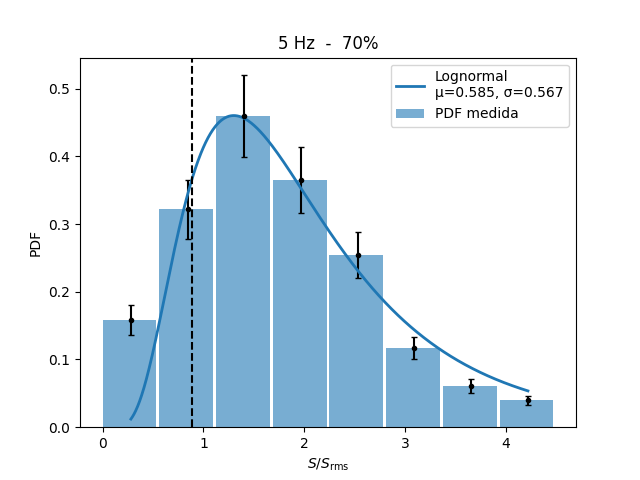
\includegraphics[width=0.98\textwidth]{Figures/08_12_2025/Distribuciones log-normal full/25}
			\captionsetup{width=0.8\textwidth}
			\subcaption{}
		\end{subfigure}
		\end{minipage}\begin{minipage}[c]{0.325\textwidth}
		\begin{subfigure}{\textwidth}
			\centering
			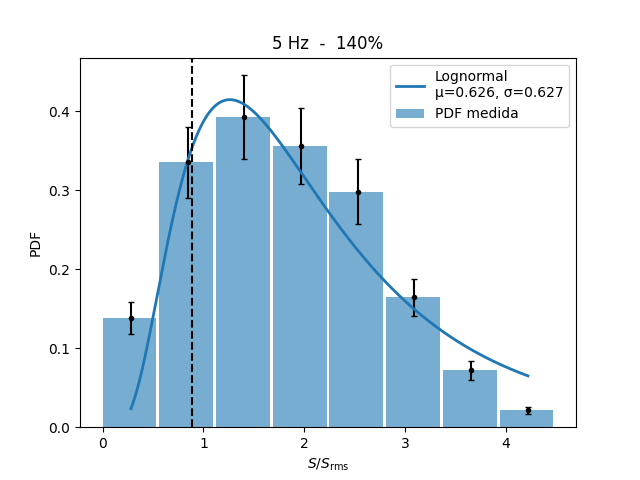
\includegraphics[width=0.98\textwidth]{Figures/08_12_2025/Distribuciones log-normal full/32}
			\captionsetup{width=0.8\textwidth}
			\subcaption{}
		\end{subfigure}
		\end{minipage} 
		
	\begin{minipage}[c]{0.325\textwidth}
		\begin{subfigure}{\textwidth}
			\centering
			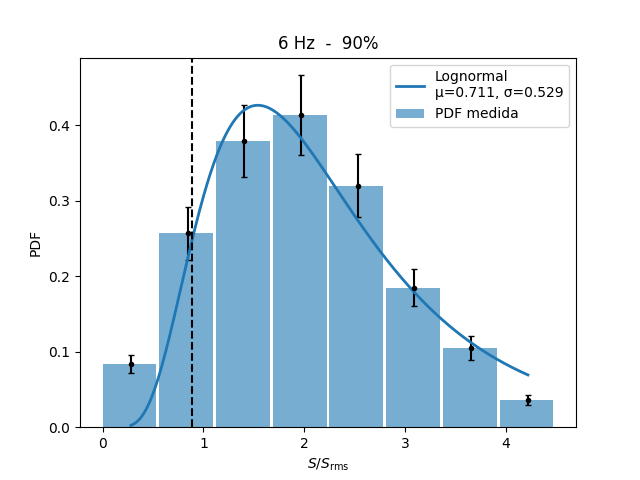
\includegraphics[width=0.98\textwidth]{Figures/08_12_2025/Distribuciones log-normal full/38}
			\captionsetup{width=0.8\textwidth}
			\subcaption{}
		\end{subfigure}
	\end{minipage}\begin{minipage}[c]{0.325\textwidth}
	\begin{subfigure}{\textwidth}
		\centering
		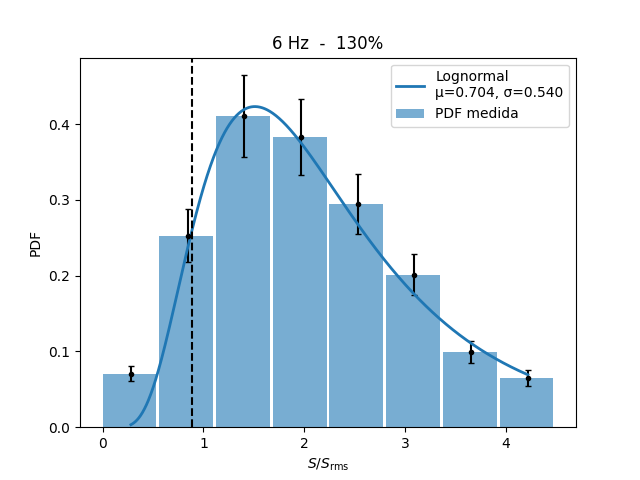
\includegraphics[width=0.98\textwidth]{Figures/08_12_2025/Distribuciones log-normal full/42}
		\captionsetup{width=0.8\textwidth}
		\subcaption{}
	\end{subfigure}
	\end{minipage}\begin{minipage}[c]{0.325\textwidth}
	\begin{subfigure}{\textwidth}
		\centering
		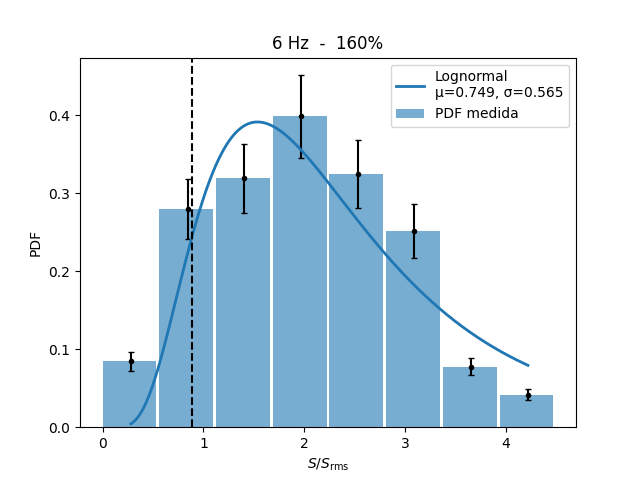
\includegraphics[width=0.98\textwidth]{Figures/08_12_2025/Distribuciones log-normal full/45}
		\captionsetup{width=0.8\textwidth}
		\subcaption{}
	\end{subfigure}
	\end{minipage}
	\caption{Algunas distribuciones de probabilidad $S/S_\text{rms}$ para las pdfs promediadas en ventanas temporales con overlap. La cantidad de bins es la raíz cuadrada de la cantidad de ondas individuales en cada histograma. Para el ajuste se tomaron los puntos centrales de los bins como coordenada x. }
	\label{fig:}
\end{figure}

Uno de los modelos propuestos por \cite{tayfunDistributionsWaveSteepness2006} es una función log-normal de la forma: 

\begin{equation}
	f(S) = \frac{1}{\sigma S\sqrt{2\pi}}\exp\left[-\frac{1}{2} \left(\frac{\ln(S) -\mu}{\sigma} \right) \right]
\end{equation}

Que funciona bien para el rango 0-3 Hz pero después se empieza a romper. Estaía bueno en mediciones más largas verificar si se rompe por la estadística de pocos puntos o es algo Físico por la no linealidades fuertes. La línea punteada se corresponde al valor teórico que debería tener el valor medio: 

\begin{equation}
	\frac{\langle S \rangle }{S_\text{rms}} = \frac{\sqrt{\pi}}{2} \approx 0.886 
\end{equation}


Un punto importante es que para calcular $S_i$ estoy usando la relación de dispersión completa de profundidad $d$. Si me limito a la aproximación de gravedad en aguas profundas del paper da mucho más puntos en $S$ pequeños como si divergiese a $S\rightarrow0$. 
 

\subsection*{Wave steepness para todos nuestros datos} 
Para todas las series temporales nuestras calculé el wave steepness medio como: 

\begin{equation}
	S_m = \langle \frac{H_i}{L(T_i)} \rangle 
\end{equation}

Usando relaciones de dispersión completa y de gravedad en aguas profundas. 

\begin{figure}[!ht]
	\begin{minipage}[c]{0.5\textwidth}
			\begin{subfigure}{\textwidth}
					\centering
					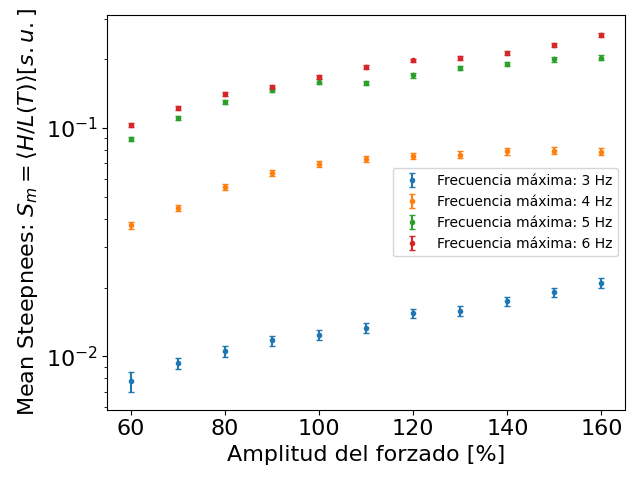
\includegraphics[width=0.978\textwidth]{Figures/08_12_2025/Mena_wave_steepness_deep_gravity.png}
					\captionsetup{width=0.8\textwidth}
					\subcaption{.}
					\label{fig:}
				\end{subfigure}
		\end{minipage}\begin{minipage}[c]{0.49\textwidth}
			\begin{subfigure}{\textwidth}
					\centering
					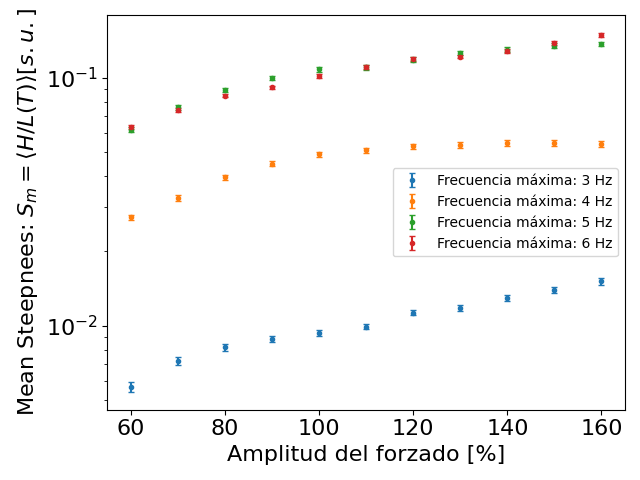
\includegraphics[width=0.978\textwidth]{Figures/08_12_2025/Mena_wave_steepness_full.png}
					\captionsetup{width=0.8\textwidth}
					\subcaption{.}
					\label{fig:}
				\end{subfigure}
		\end{minipage}
	\caption{}
	\label{fig:}
\end{figure}

Para la de aguas profundas solo en gravedad se distinguen bien las cuatro bandas de frecuencias y se ve que siempre $S_m$ aumenta al aumentar la energía inyectada. Para la completa las últimas dos bandas de frecuencias tienden a dar lo mismo. La banda de 0-4 Hz llega a saturar bastante rápido. 


Estaría bueno probar si cambia esto usando los valores medios que salen del ajuste por la log-normal. 




\section{Parámetros de las cascadas en función del wave steepness} 

Lo último que probé fue ver cómo se relacionan los parámetros de las cascadas con el wave steepness (a modo de unión entre las distintas bandas). % v 

\begin{figure}[th!]
	\centering
	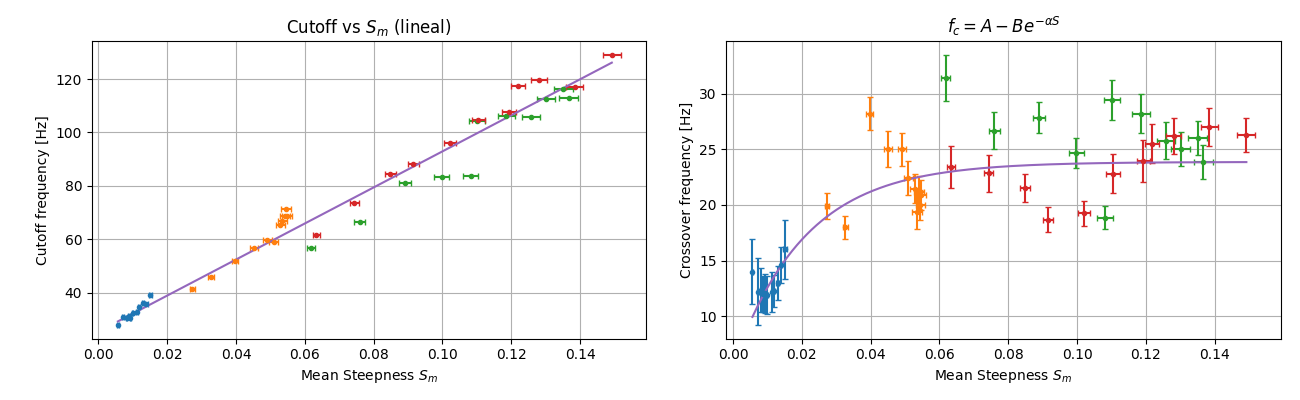
\includegraphics[width=0.9897\linewidth]{Figures/08_12_2025/Correlación_parámetros}
	\caption{Correlación del mean wave steepness con el cutoff y frecuencia de corte de los espectros.}
	\label{fig:correlacionparametros}
\end{figure}

El cutoff pareciera aumentar linealmente mientras que la frecuencia de cruce parece subir exponencialmente hasta saturar en el doble de la frecuencia \textit{lineal}. Los parámetros de los ajuste son:  
\begin{itemize}
	\item Cutoff: Pendiente = (674.977 $\pm$ 0.004) Hz y Ordenada = (25.408 $\pm$ 0.00010) Hz. 
	\item Exponencial: A = (23.863 $\pm$ 0.369) Hz, B = (18.263 $\pm$ 1.612) Hz y $\alpha$ = (48.125 $\pm$ 7.463). 
\end{itemize}

También estaría bueno hacer mediciones enfocadas a ver si estas suposiciones son coherentes. 



\section{Transitorios} 
El otro tipo de mediciones que hice fue con una serie temporal en el forzado que es ruido con una envolvente de la forma $1-e^{-t/\tau}$. Los resultados son los siguientes:  

\begin{figure}[th!]
	\centering
	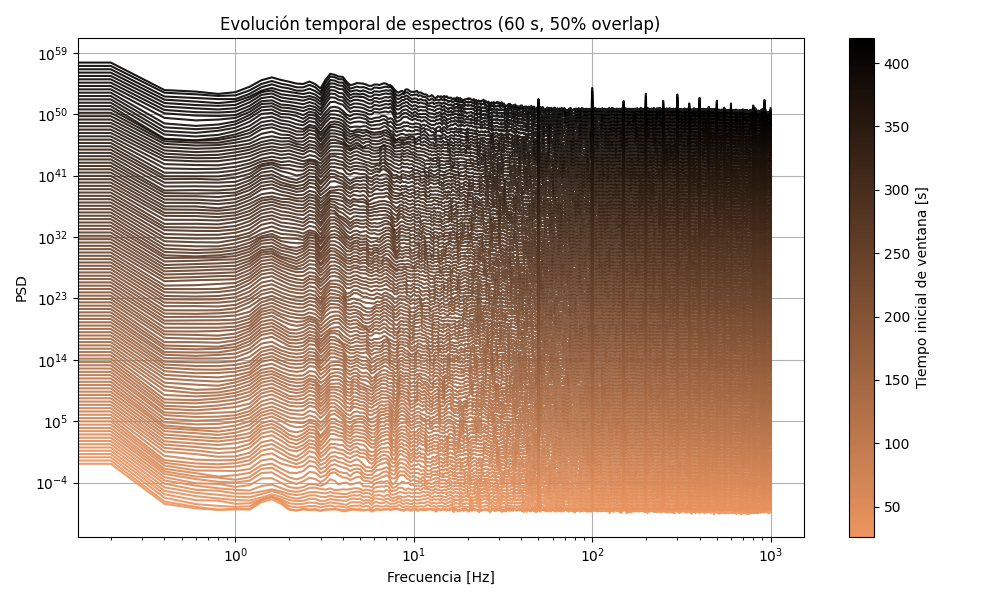
\includegraphics[width=0.87\linewidth]{Figures/08_12_2025/Transitorio_0_4_Hz}
	\caption{PSDs para el forzado entre 0 y 4 Hz.}
	\label{fig:transitorio04hz}
\end{figure} 

\begin{figure}[th!]
	\centering
	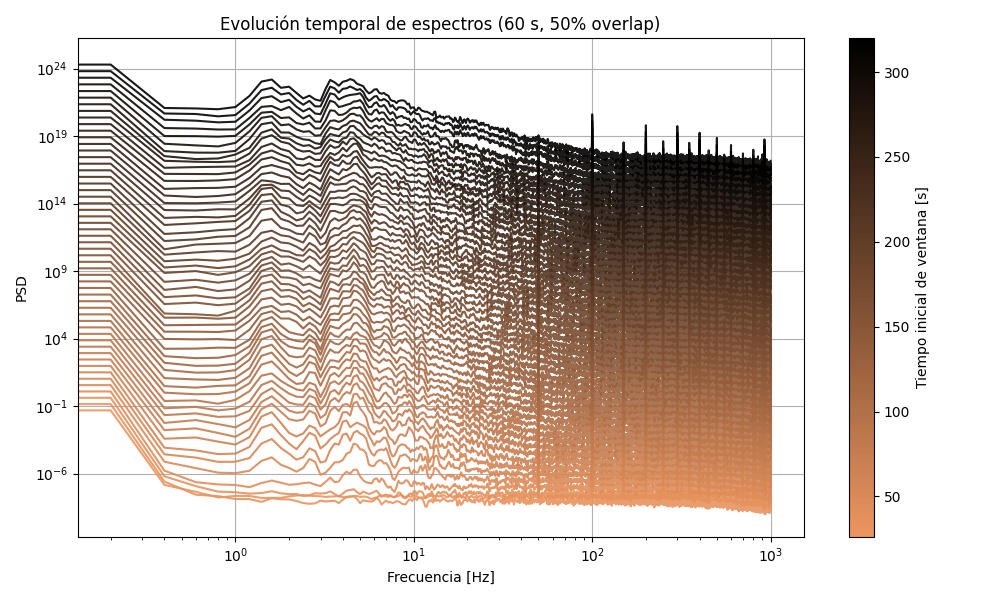
\includegraphics[width=0.87\linewidth]{Figures/08_12_2025/Transitorio_0_6_Hz}
	\caption{PSDs para el forzado entre 0 y 6 Hz.}
	\label{fig:transitorio06hz}
\end{figure}


\section{¿Observación de Sandpiles en el transitorio?} 
Por último, en el espectro de 0-4 Hz parecieran observarse las sandpiles, ya que se acumula energía en frecuencias bajas y después salta al doble, y así sucesivamente. 

\begin{figure}[th!] % H 
	\centering
	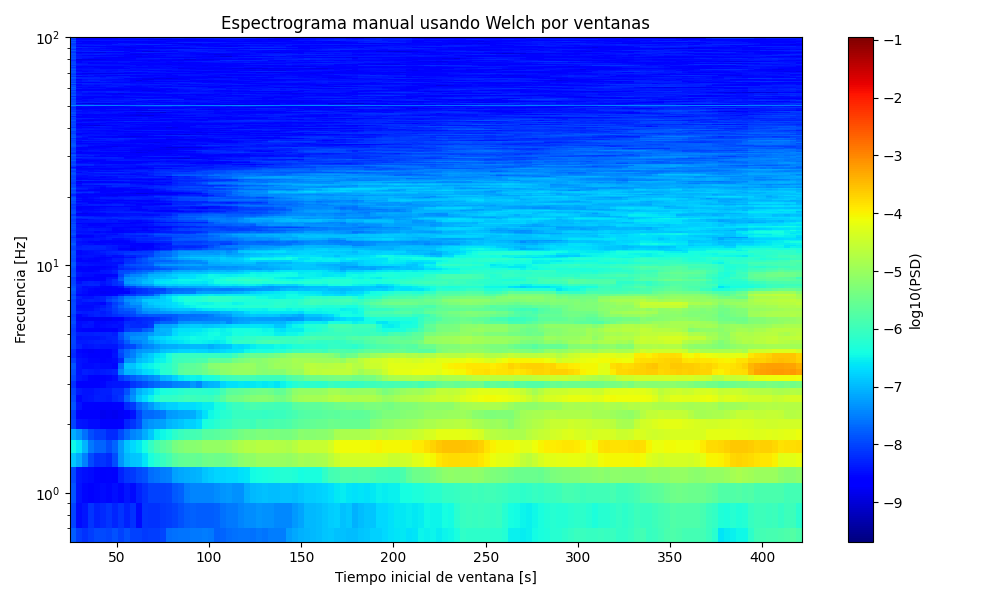
\includegraphics[width=0.7\linewidth]{Figures/08_12_2025/Sandpiles_0_4_Hz}
	\caption{Espectrograma de la señal transitoria con el forzado entre 0 y 4 Hz.}
	\label{fig:sandpiles04hz}
\end{figure}

Habría que hacer algún otro análisis para verificar si son estos, y estudiar el periodo en que se prenden y se apagan las distintas frecuencias. 



